\appendix
\FloatBarrier
\centering
\section*{appendix}


%PROTOTYPE ET STARTER HER
%\subsection*{f�rste prototype}
%\centering

\begin{figure}[ht]
\centering
   	
\includegraphics{1.Prototype/Login_Vindue}
    \caption{Login Vindue 1.prototype}
    \label{login1}
\end{figure}
\begin{figure}[ht]
\centering
   	
\includegraphics{1.Prototype/Login_Vindue_Info}
    \caption{Login vindue med info 1.Prototype}
    \label{login1info}
\end{figure}
\begin{figure}[ht]
\centering
	\includegraphics[height= 185px]{1.Prototype/Status_Vindue}
    \caption{Status vindue 1.Prototype}
    \label{ssowindow1}
\end{figure}

%PROTOTYPE TO STARTER HER
\FloatBarrier
%\subsection*{anden prototype}
%\centering

\begin{figure}[ht]
\centering
	
\includegraphics{2.Prototype/Login_Vindue}
    \caption{Login Vindue 2.Prototype}
    \label{login2}
\end{figure}
\begin{figure}[ht]
\centering
	
\includegraphics{2.Prototype/Login_Vindue_Info}
    \caption{Login Vindue med info 2.Prototype}
    \label{login2info}
\end{figure}
\begin{figure}[ht]
\centering
	\includegraphics[height= 200px]{2.Prototype/Status_Vindue}
    \caption{Status Vindue 2.Prototype}
    \label{ssowindow2}
\end{figure}
\begin{figure}[ht]
\centering
	
\includegraphics{2.Prototype/TrayIcon}
    \caption{Tray Icon 2.Prototype}
    \label{tray2}
\end{figure}
\begin{figure}[ht]
\centering
	
\includegraphics{2.Prototype/TrayIconMenu}
    \caption{Tray Icon menu 2.Prototype}
    \label{tray2menu}
\end{figure}

%PROTOTYPE TRE STARTER HER
\FloatBarrier
%\subsection*{Tredje prototype}
%\centering

\begin{figure}[ht]
\centering
   	
\includegraphics{3.Prototype/Login_Vindue}
    \caption{Login Vindue 3.Prototype}
    \label{login3}
\end{figure}


\begin{figure}[ht]
\centering
	
\includegraphics[height= 110px]{3.Prototype/Login_Vindue_Info}
    \caption{Login Vindue info 3.Prototype}
    \label{login3info}
\end{figure}
\begin{figure}[ht]
\centering
	\includegraphics{3.Prototype/Status_Vindue}
    \caption{Status Vindue 3.Prototype}
    \label{ssowindow3}
\end{figure}
\begin{figure}[ht]
\centering
	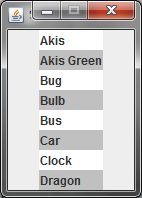
\includegraphics{3.Prototype/Add_Vindue}
    \caption{Add Vindue 3.Prototype}
    \label{add3}
\end{figure}
\begin{figure}[ht]
\centering
	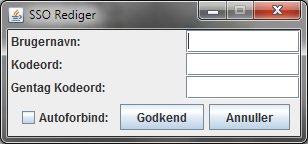
\includegraphics{3.Prototype/Edit_Vindue}
    \caption{Edit Vindue 3.Prototype}
    \label{edit3}
\end{figure}
\begin{figure}[ht]
\centering
	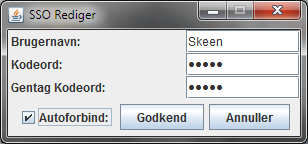
\includegraphics{3.Prototype/Edit_Vindue_Info}
    \caption{Edit Vindue Info 3.Prototype}
    \label{edit3info}
\end{figure}
\begin{figure}[ht]
\centering
	
\includegraphics{3.Prototype/TrayIcon}
    \caption{Tray Icon 3.Prototype (2. ikon fra venstre)}
    \label{tray3}
\end{figure}
\begin{figure}[ht]
\centering
	
\includegraphics{3.Prototype/TrayIconMenu}
    \caption{Tray Icon menu 3.Prototype}
    \label{tray3menu}
\end{figure}

\begin{figure}[ht]
\centering
	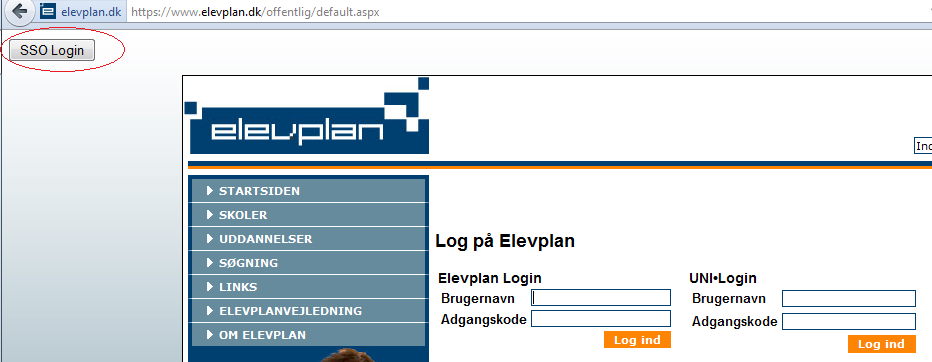
\includegraphics[height= 150px]{3.Prototype/SSO_Login_Button}
    \caption{SSO Login Button 3.Prototype}
    \label{ssologinbutton}
\end{figure}
\begin{figure}[ht]
\centering
	
\includegraphics[height= 100px]{3.Prototype/404}
    \caption{Fejl: 404 3.Prototype}
    \label{fejl404}
\end{figure}

\begin{figure}[ht]
\centering
	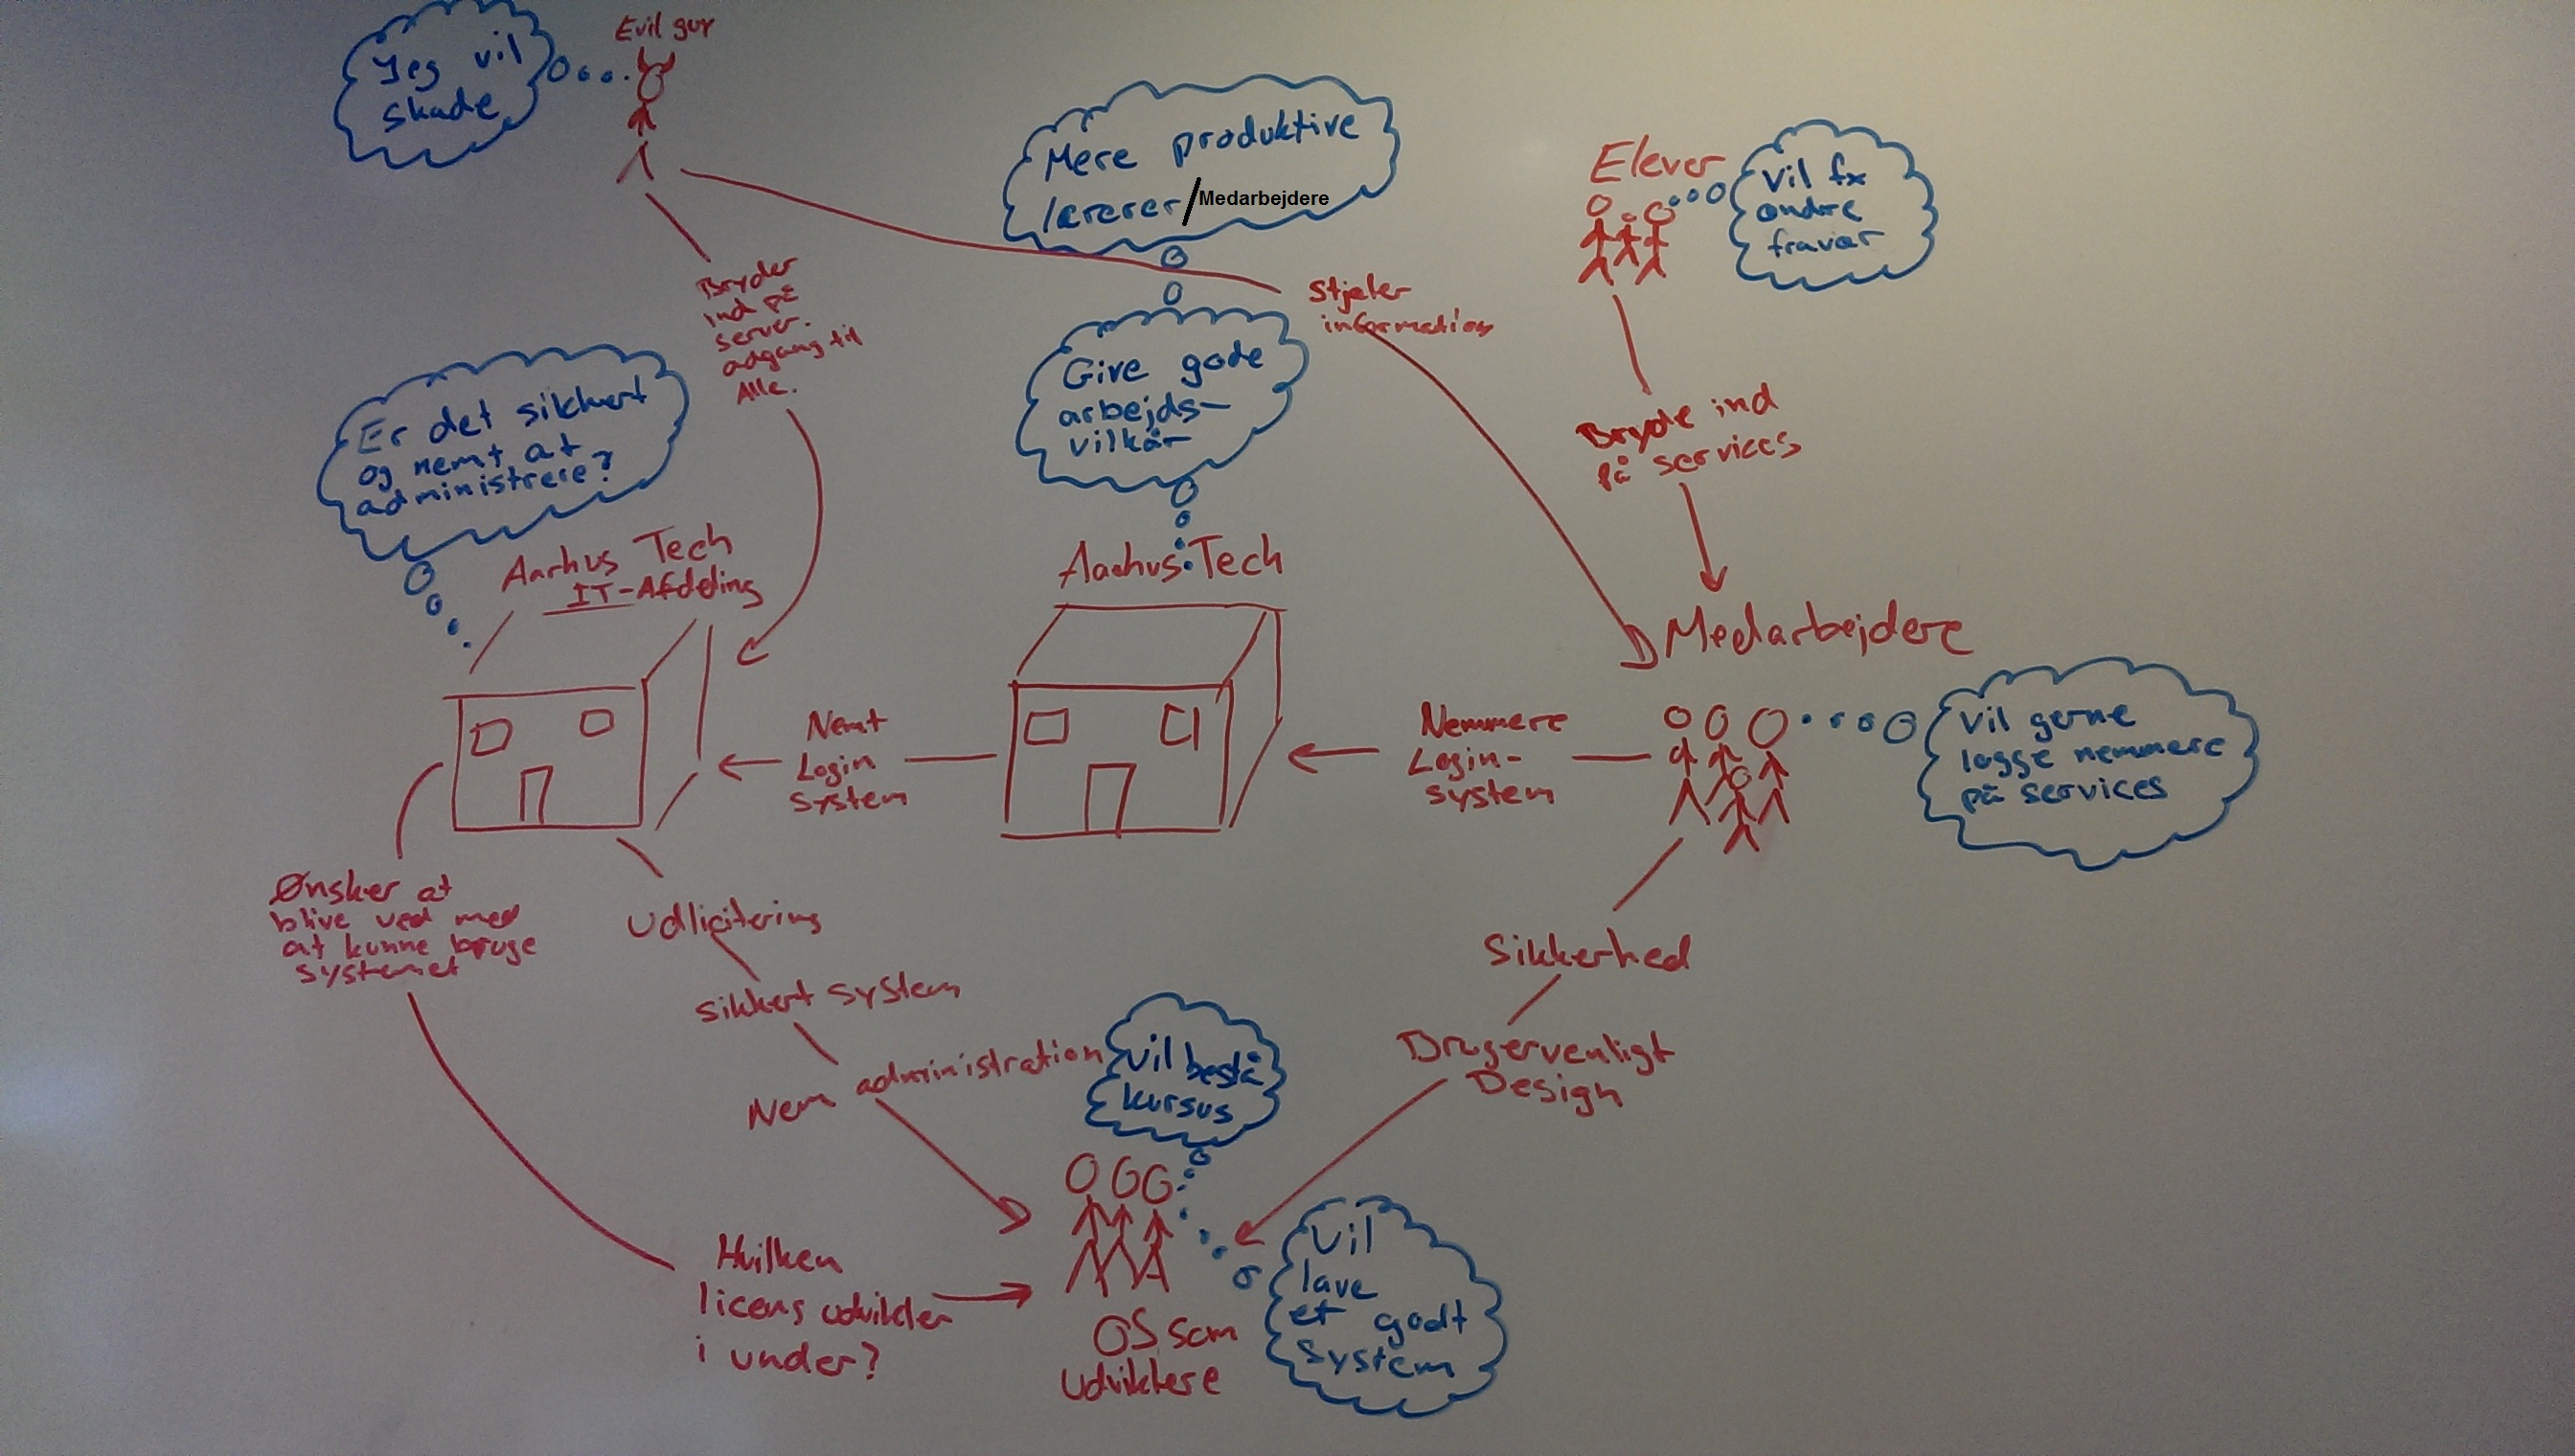
\includegraphics[height= 235px]{Rich_Picture}
    \caption{Rich Picture}
    \label{richpicture}
\end{figure}

\FloatBarrier

{\bf Backlog}
Grundet projektets slutning, er disse ting ikke blevet
implementeret;
\begin{itemize}
\item Kryptering af key-value information, p� databasen.
\item Integerering med Active Directory (login proces)
\item Integerering med Active Directory Dom�ne Server (bruger synkronisering)
\item Redesign eller fjernelse af 'Opdater' knappen
\item Ordenlig injection af HTML i proxy svar (vha. jsoup)
\item Ordenlig implementering af VPN support, og wifi
\item Status Checking af webservices
\item Mulighed for disconnection af webservices
\item Mulighed for autogenerede short-cuts p� skrivebordet
\item Underst�ttelse af h�jre-click context menu (p� status vinduet)
\item Vedholdne computer specifikke configurationer, f.eks. vindue st�rrelse
\item Ydereligere refactorering og oprydning af source koden
\end{itemize}


%interview pdfs
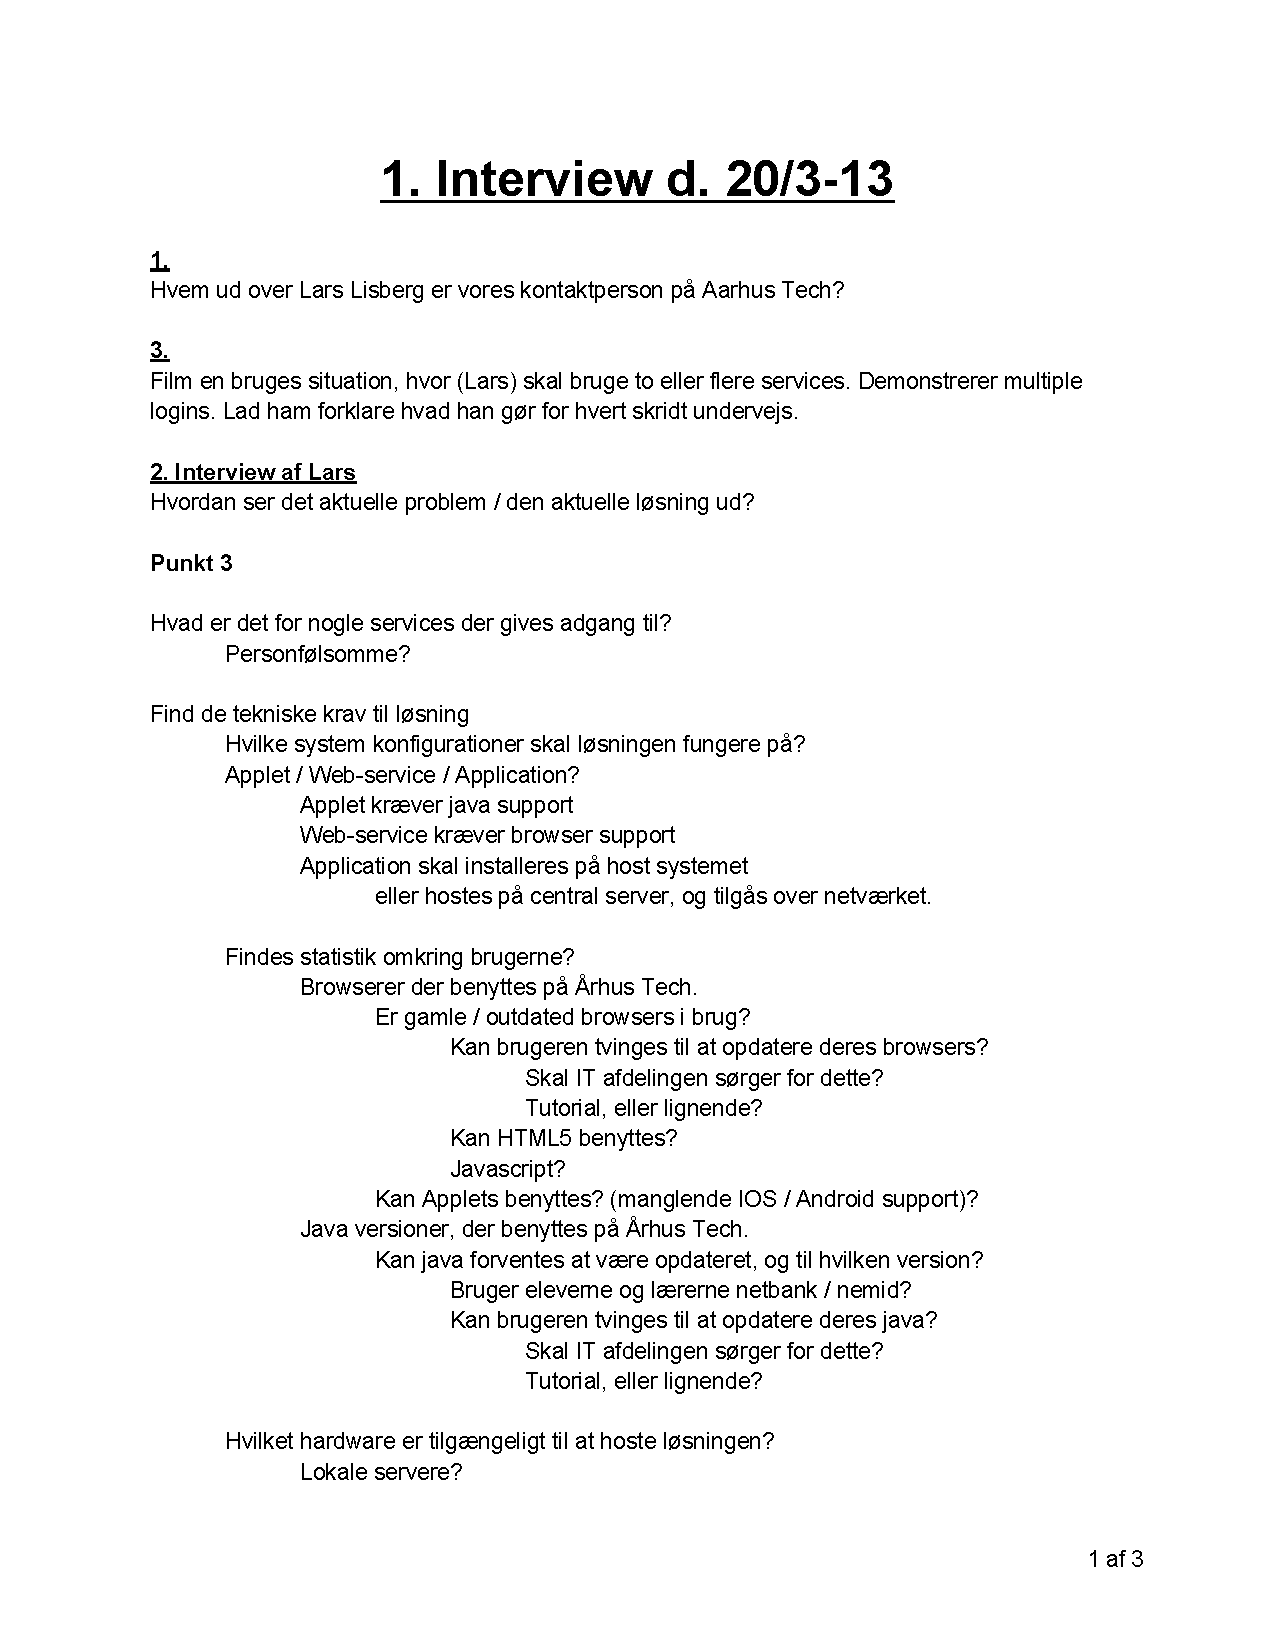
\includepdf[pages={1,2,3}]{gfx/1_interview.pdf}
\label{interview1}

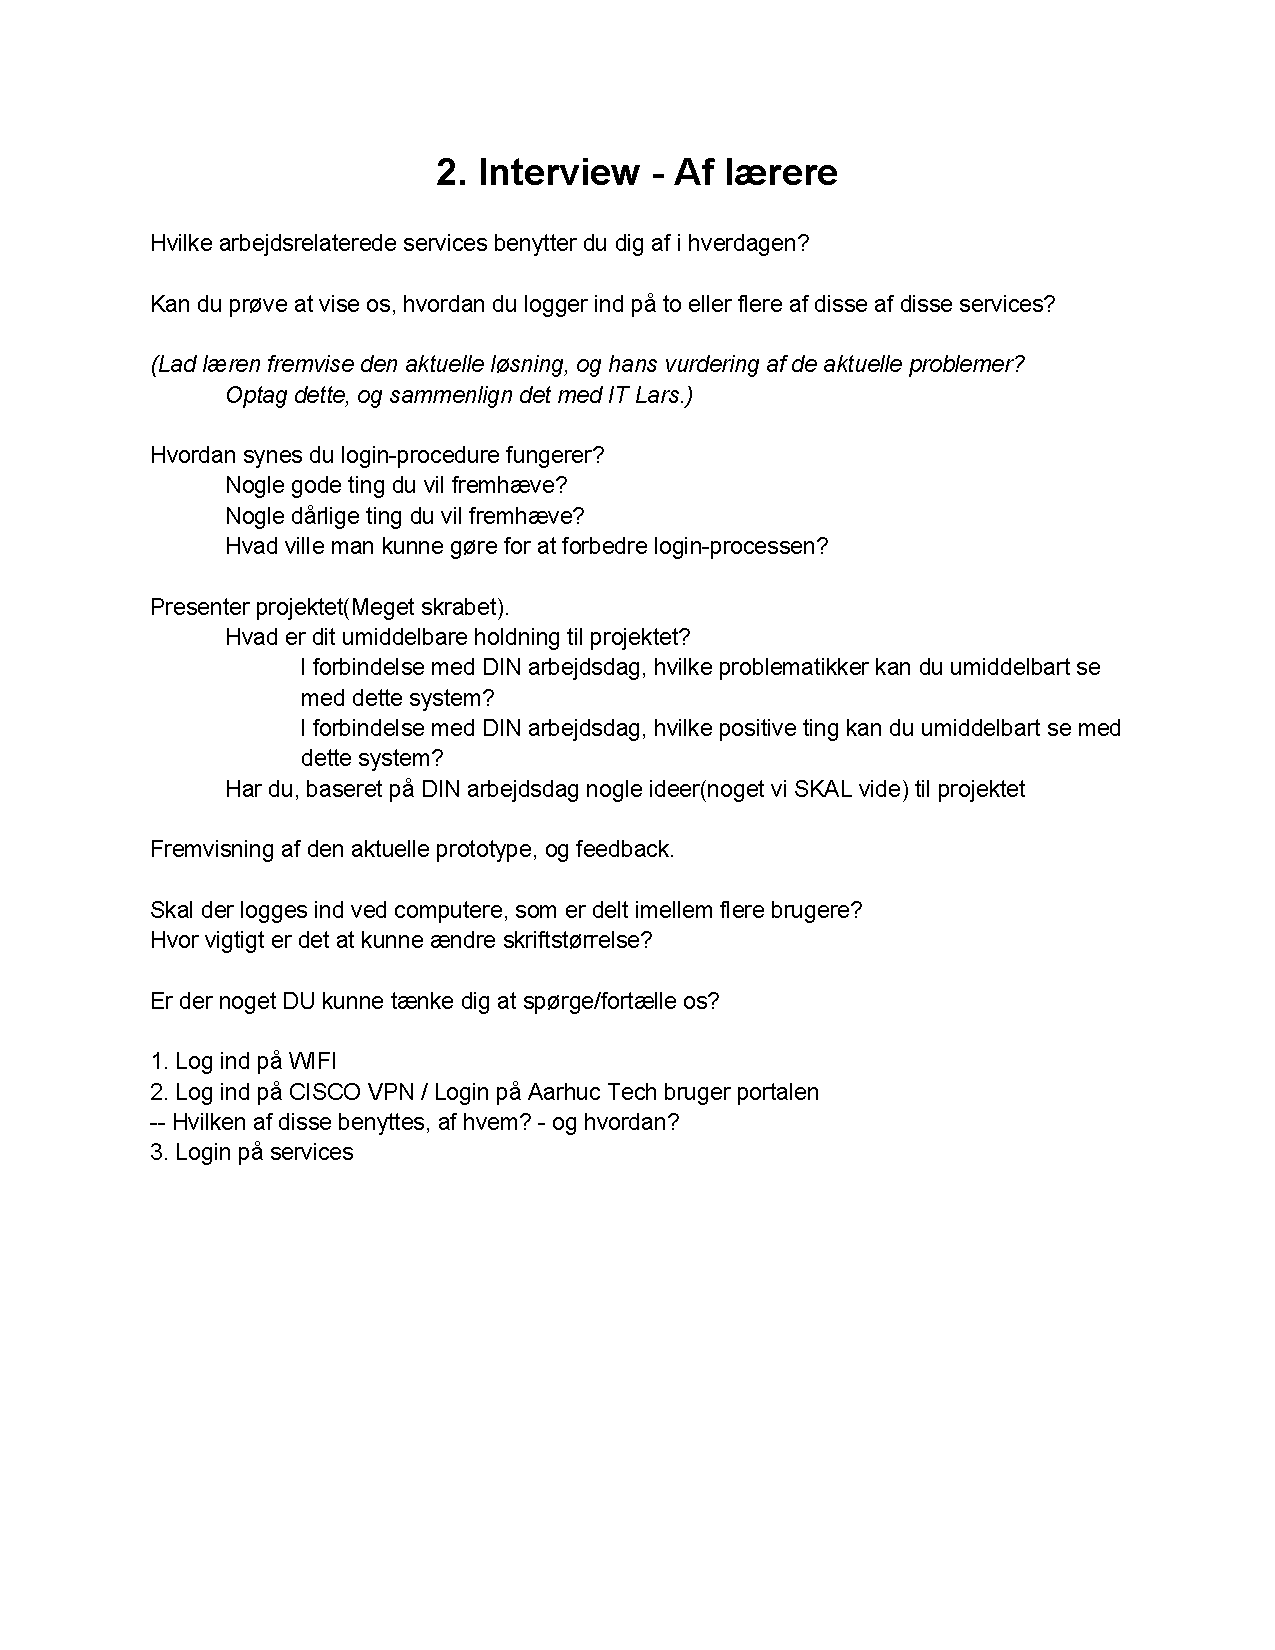
\includepdf[pages={1}]{gfx/2_interview.pdf}
\label{interview2}

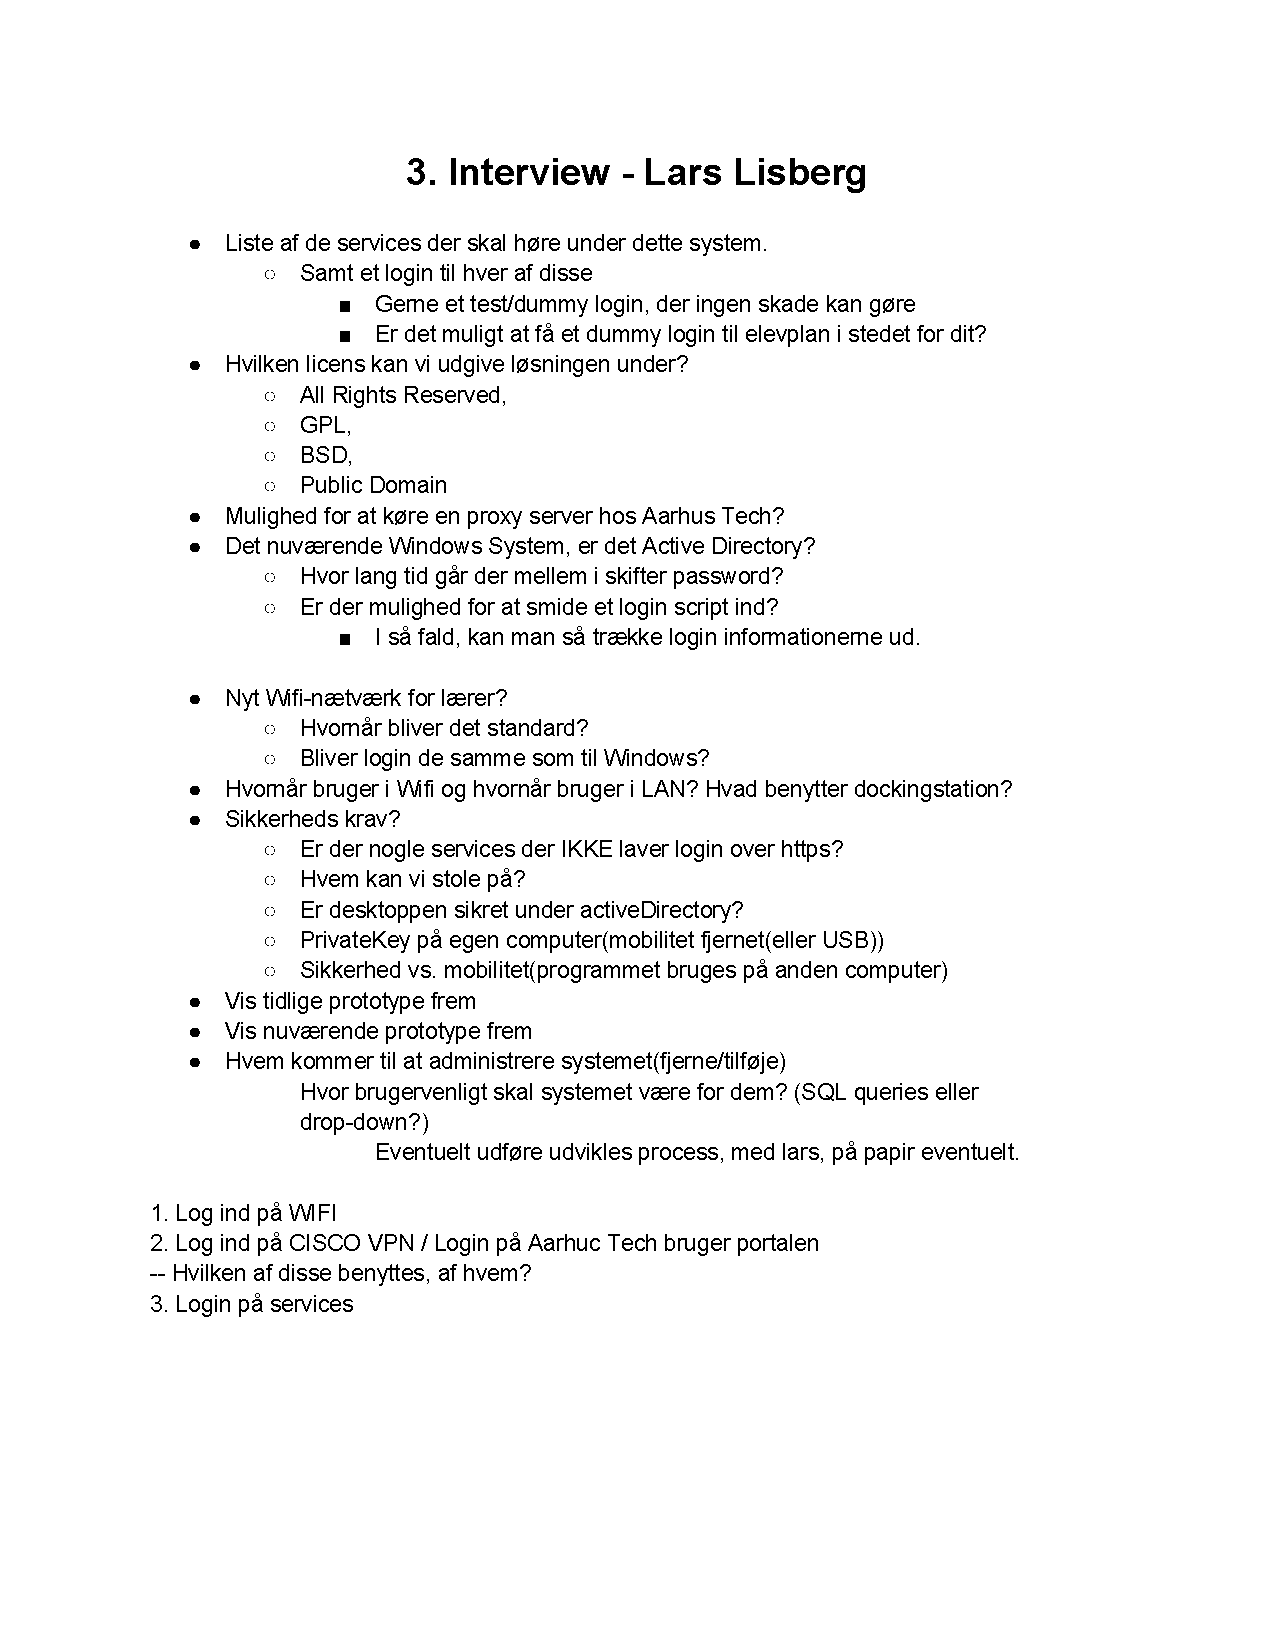
\includepdf[pages={1}]{gfx/3_interview.pdf}
\label{interview3}
